\documentclass[a4paper, 11pt]{article}
\usepackage[UTF8]{ctex}
\usepackage{amsmath}
\usepackage{graphicx}
\usepackage{pythonhighlight}
\usepackage{geometry}
\usepackage{listings}
\geometry{scale=0.8}
\linespread{1.5}
\usepackage{hyperref}

\title{	
\normalfont \normalsize
\textsc{School of Data and Computer Science, Sun Yat-sen University} \\ [25pt] %textsc small capital letters
\rule{\textwidth}{0.5pt} \\[0.4cm] % Thin top horizontal rule
\huge  E04 Futoshiki Puzzle ( Forward Checking)\\ % The assignment title
\rule{\textwidth}{2pt} \\[0.5cm] % Thick bottom horizontal rule
\author{17341175 徐志成}
\date{\normalsize\today}
}

\begin{document}
\maketitle
\tableofcontents
\newpage

\section{Futoshiki}
Futoshiki is a board-based puzzle game, also known under the name Unequal. It is playable on a square board having a given fixed size ($4\times4$ for example).

The purpose of the game is to discover the digits hidden inside the board's cells; each cell is filled with a digit between 1 and the board's size. On each row and column each digit appears exactly once; therefore, when revealed, the digits of the board form a so-called Latin square.

At the beginning of the game some digits might be revealed. The board might also contain some inequalities between the board cells; these inequalities must be respected and can be used as clues in order to discover the remaining hidden digits.

Each puzzle is guaranteed to have a solution and only one.

You can play this game online: \url{http://www.futoshiki.org/}.
\begin{figure}[h]
  \centering
  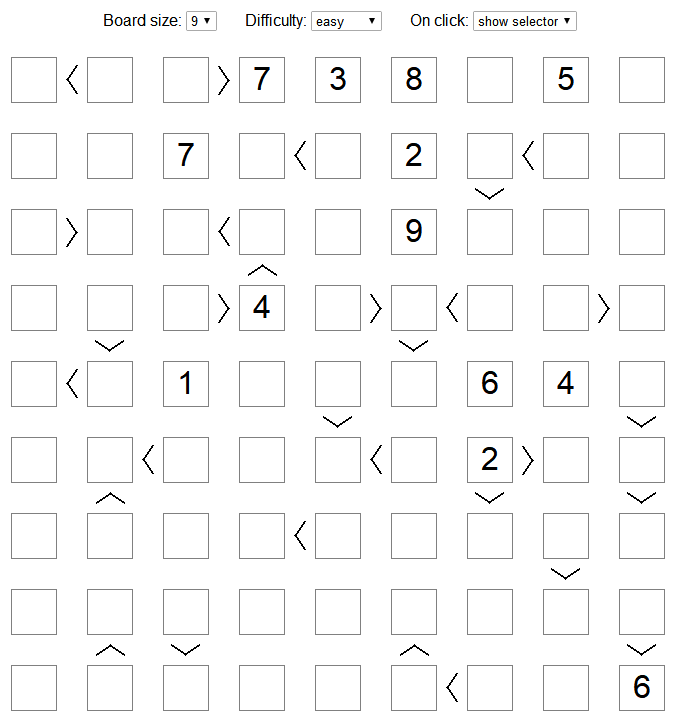
\includegraphics[width=7.5cm]{Pic/futoshiki1}
  \qquad
  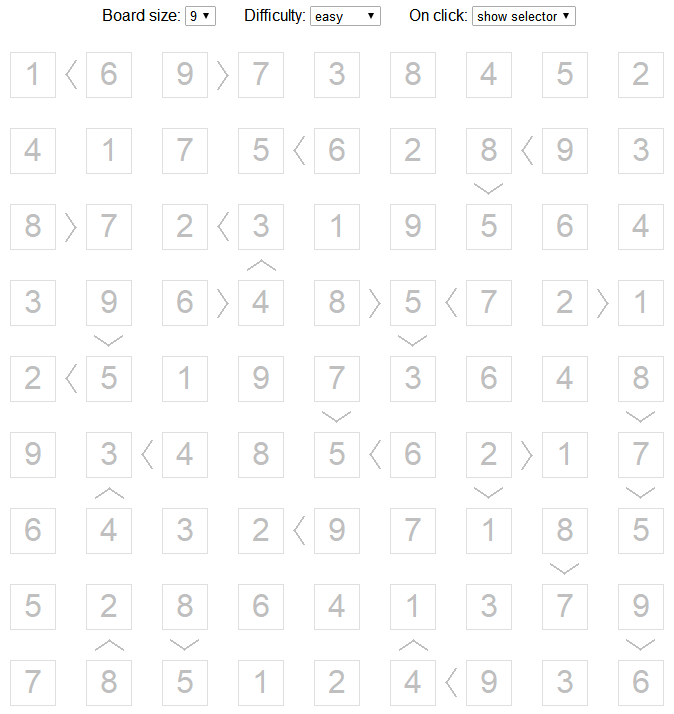
\includegraphics[width=7.5cm]{Pic/futoshiki2}
  \label{fig:puzzle}
  \caption{An Futoshiki Puzzle}
\end{figure}

\section{Tasks}


\begin{enumerate}
\item Please solve the above Futoshiki puzzle ( Figure \ref{fig:puzzle} ) with forward checking algorithm.
\item Write the related codes and take a screenshot of the running results in the file named \textsf{E04\_YourNumber.pdf}, and send it to \textsf{ai\_201901@foxmail.com}.

\end{enumerate}
\section{Codes}
\begin{python}
import queue

size = 0
def DWO(values, compare, x, y, num):
    constraints = [[False for _ in range(size)] for _ in range(2)]
    FCQueue = queue.Queue()
    # 0 means row, 1 means column
    FCQueue.put((0, x))
    FCQueue.put((1, y))
    constraints[0][x] = True
    constraints[1][y] = True
    while (not FCQueue.empty()):
        index, n = FCQueue.get()
        constraints[index][n] = False
        for a in range(size):
            if (index == 0):
                x, y = n, a
            else:
                x, y = a, n
            temp = list(values[x][y])
            for now in temp:
                if (check(values, compare, index, n, x, y, now) == False):
                    values[x][y] = [value for value in values[x][y] if value != now]
                    if (not values[x][y]):
                        return True
                    else:
                        FCQueue.put((index, n))
                        constraints[index][n] = True
                        if (constraints[1 - index][a] == False):
                            FCQueue.put((1 - index, a))
                            constraints[1 - index][a] = True

    return False


def compare_fail(values, compare, x, y, now):
    small, large = compare
    if ((x, y) in small):
        for a, b in small[(x, y)]:
            for value in values[a][b]:
                if (now < value):
                    return False
        return True
    if ((x, y) in large):
        for a, b in large[(x, y)]:
            for value in values[a][b]:
                if (now > value):
                    return False
        return True
    return False


def dfs(values, compare, index, n, now, visited):
    if now == size:
        return True
    if (index == 0):
        x, y = n, now
    else:
        x, y = now, n

    for value in values[x][y]:
        if (visited[value - 1] or compare_fail(values, compare, x, y, value)):
            continue
        visited[value - 1] = True
        if (dfs(values, compare, index, n, now + 1, visited)):
            return True
        visited[value - 1] = False

    return False


def read(string):
    global size
    chess_board = []
    small, large = {}, {}
    f=open(string)
    line = f.readline().strip('\n')
    size = int(line)
    print(size)
    for _ in range(size):
        line = f.readline().strip('\n')
        if line == '':
            continue
        nums = [int(num) for num in line.rstrip().split(' ')]

        chess_board.append(nums)
    for i in chess_board:
        print(i)

    lines = f.readlines()
    for line in lines:
        line = line.strip('\n')
        if line == '':
            continue
        a, b, c, d = [int(num) for num in line.rstrip().split(' ')]
        left, right = (a, b), (c, d)
        if (left in small):
            small[left].append(right)
        else:
            small[left] = [right]
        if (right in large):
            large[right].append(left)
        else:
               large[right] = [left]

    compare = (small, large)
    return chess_board, compare


def check(values, compare, index, n, x, y, value):
    visited = [False for _ in range(size)]
    before = list(values[x][y])
    values[x][y] = [value]
    flag = dfs(values, compare, index, n, 0, visited)
    values[x][y] = before
    return flag



def copy_temp(a):
    b = []
    for row in a:
        temp_row = []
        for col in row:
            temp = list(col)
            temp_row.append(temp)
        b.append(temp_row)

    return b


def initial(chess_board, compare):
    values = []
    assign = [[False for _ in range(size)] for _ in range(size)]
    for row in chess_board:
        value_row = []
        for index in row:
            if (index == 0):
                value = [a for a in range(1, size + 1)]
                value_row.append(value)
            else:
                value_row.append([index])

        values.append(value_row)

    for a in range(size):
        for b in range(size):
            if (chess_board[a][b] != 0):
                assign[a][b] = True
                DWO(values, compare, a, b, chess_board[a][b])
    return (values, assign)


def assginment(values, assign):
    Min = 999
    x, y = -1, -1
    for a in range(size):
        for b in range(size):
            l = len(values[a][b])
            if (assign[a][b] == False and l < Min):
                Min = l
                x = a
                y = b

    return (x, y)


def printf(chess_board):
    for row in chess_board:
        for index in row:
            print(str(index), end=' ')
        print('')


def FC(values, compare, assign, chess_board):
    (x, y) = assginment(values, assign)
    if ((x, y) == (-1, -1)):
        return True

    assign[x][y] = True
    members = list(values[x][y])
    for num in members:
        chess_board[x][y] = num
        temp_values = copy_temp(values)
        values[x][y] = [num]
        if (DWO(values, compare, x, y, num) == False):
            flag = FC(values, compare, assign, chess_board)
            if (flag):
                return True

        values = copy_temp(temp_values)

    assign[x][y] = False
    return False


def run(string):
    chess_board, compare = read(string)
    values, assign = initial(chess_board, compare)
    dd = FC(values, compare, assign, chess_board)
    if (dd):
        printf(chess_board)



string = 'dataE04_2.txt'
run(string)


\end{python}


\section{Results}
\begin{figure}[h]
  \centering
  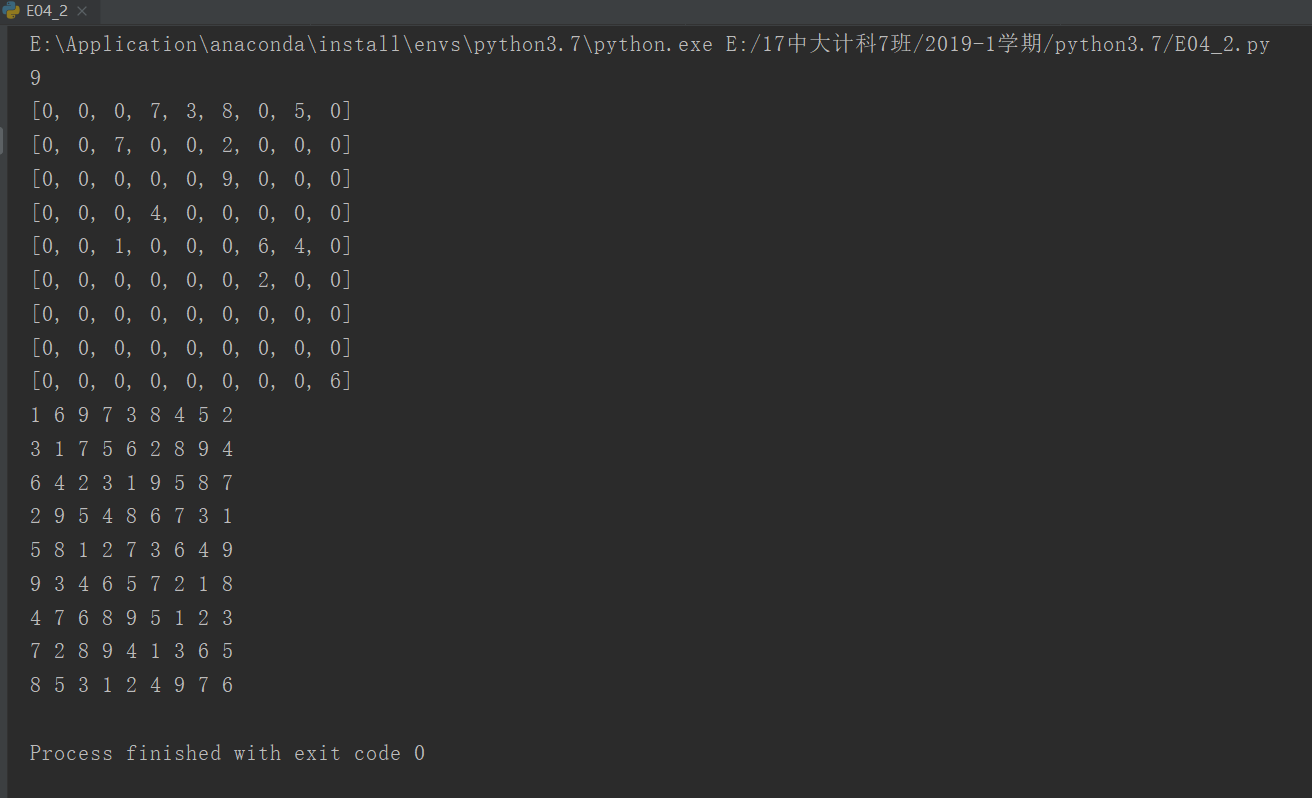
\includegraphics{Pic/result.png}
  
  \caption{result}
\end{figure}

%\clearpage
%\bibliography{E:/Papers/LiuLab}
%\bibliographystyle{apalike}
\end{document} 
%%% Local Variables:
%%% mode: latex
%%% TeX-master: t
%%% End:
